\section{Aufbau der Komponentenarchitektur}
In dem letzten Abschnitt wurden die elementaren Funktionen des Regelkreises, wie die Peripherieinteraktion und der Signalfluss, implementiert. Um eine effiziente Versuchsdurchführung zu ermöglichen, müssen allerdings weitere Funktionalitäten bereitstehen. Einerseits müssen einzelne Elemente des Regelkreises während der Ausführung konfigurierbar sein. Beispielsweise soll zwischen unterschiedlichen Regler umgeschaltet werden und einzelne Parameter geändert werden können. Andererseits müssen die gemessenen und berechneten Werte des Signalflusses an einen Entwicklungsrechner übertragen werden. Dort werden die Daten visualisiert und für eine spätere Analyse gespeichert.
Folglich muss ein Kommunikationskonzept implementiert werden, um Daten zwischen der Ziel- und Entwicklungsplattform auszutauschen. Um die Berechnung des Regelkreises und die Kommunikationsaufgaben voneinander zu trennen, wird eine Komponentenarchitektur eingeführt \cite[S. 279 ff.]{Wietzke1}. Die erste Komponente, welche als Regelungskomponente bezeichnet wird, führt die Berechnung des Signalflusses und die Interaktion mit den Peripheriegeräten durch. Des Weiteren übernimmt sie die logische Steuerung der Versuchsabläufe. Die Kommunikationskomponente ist für die Verbindung mit dem Entwicklungsrechner verantwortlich und ermöglicht den Datenaustausch zwischen den beiden Plattform. Hierfür wird ein TCP/IP-Server verwendet.
\begin{figure}[!h]
\centering
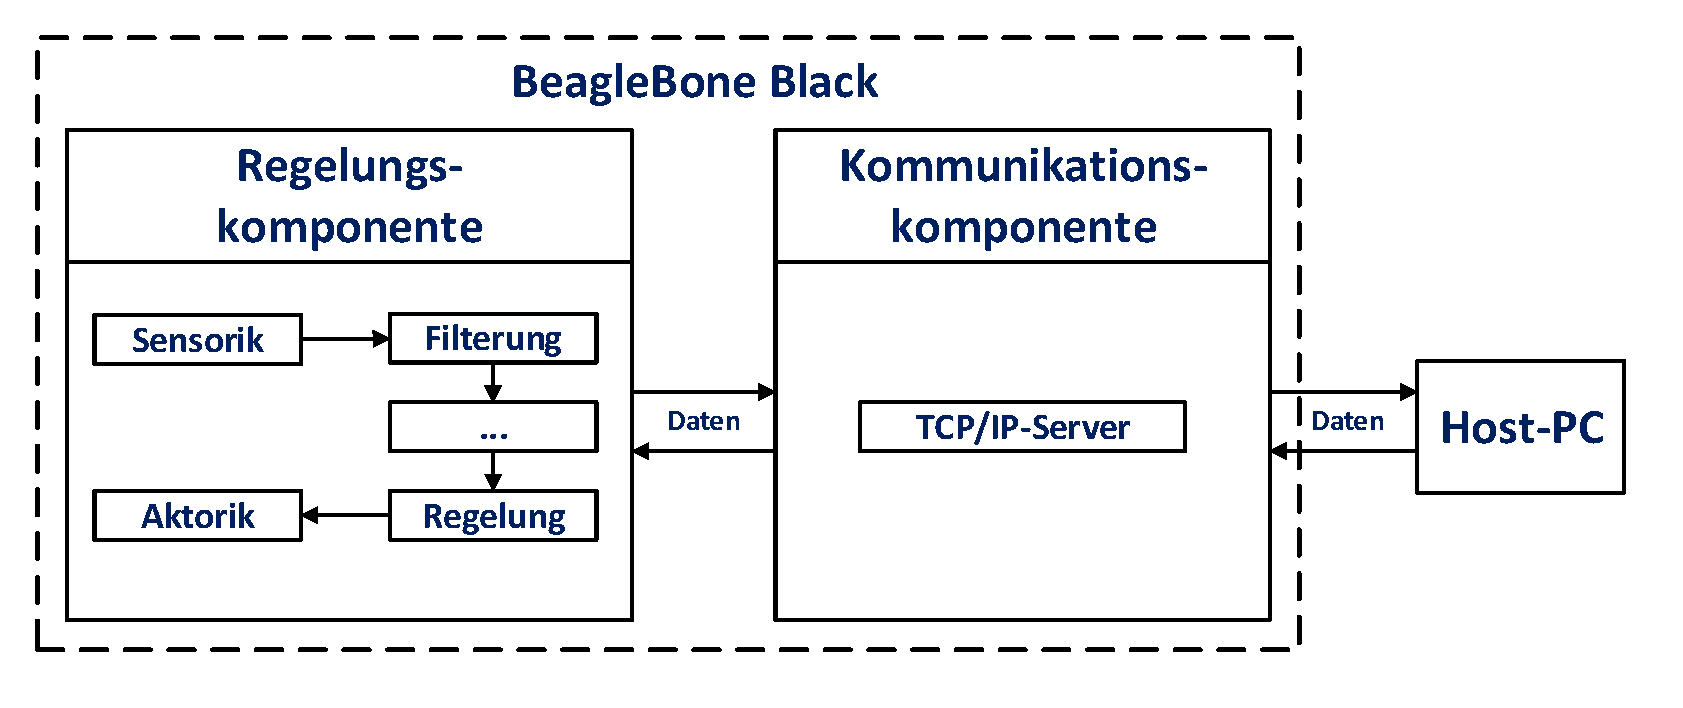
\includegraphics[width=\linewidth]{img/SW_1_KA_BSB.pdf}
\caption{Blockschaltbild Gesamtsystem}
\end{figure}
Durch die Verwendung der Komponentenarchitektur entstehen einige Vorteile. Zunächst können die beiden Komponenten in unterschiedlichen Threads ausgeführt werden, wodurch die Bearbeitung der beiden Aufgabenbereiche zum Großteil entkoppelt wird. Der Datenaustausch zwischen den Komponenten reduziert sich auf eine kontrollierte Schnittstelle, wodurch die Fehleranfälligkeit des Gesamtsystems minimiert wird. Zudem können die Aufgaben priorisiert werden, da der Scheduler eine preemptive Round-Robin-Strategie verfolgt \cite[S. 19]{Wietzke1}. Somit kann die Ausführung der Regelungskomponente, welche für die Bearbeitung der zeit- und sicherheitsrelevanten Aufgaben zuständig ist, gegenüber der Kommunikationseinheit priorisiert werden. Hieraus resultiert, dass das Zeitverhalten der Regelung als deterministisch angenommen werden kann. 

Für die Implementierung wird das Interface \textit{IRunnable} definiert, welches virtuelle Methoden zur Initialisierung und Ausführung der Komponenten vorschreibt. Diese Schnittstelle wird von der abstrakten Klasse \textit{AComponentBase} geerbt, welche Membervariablen zum Datenaustausch besitzt. Die letzendlichen Komponenten werden in Form der beiden Klassen \textit{CControlComp} und \textit{CCommComp} realisiert. Die Erzeugung der Threads erfolgt mit Hilfe der Klasse \textit{CThread}, deren Instanz als Trägerobjekte der Threads agieren \cite[S. 108 ff.]{Wietzke1}.
\begin{figure}[!h]
\centering
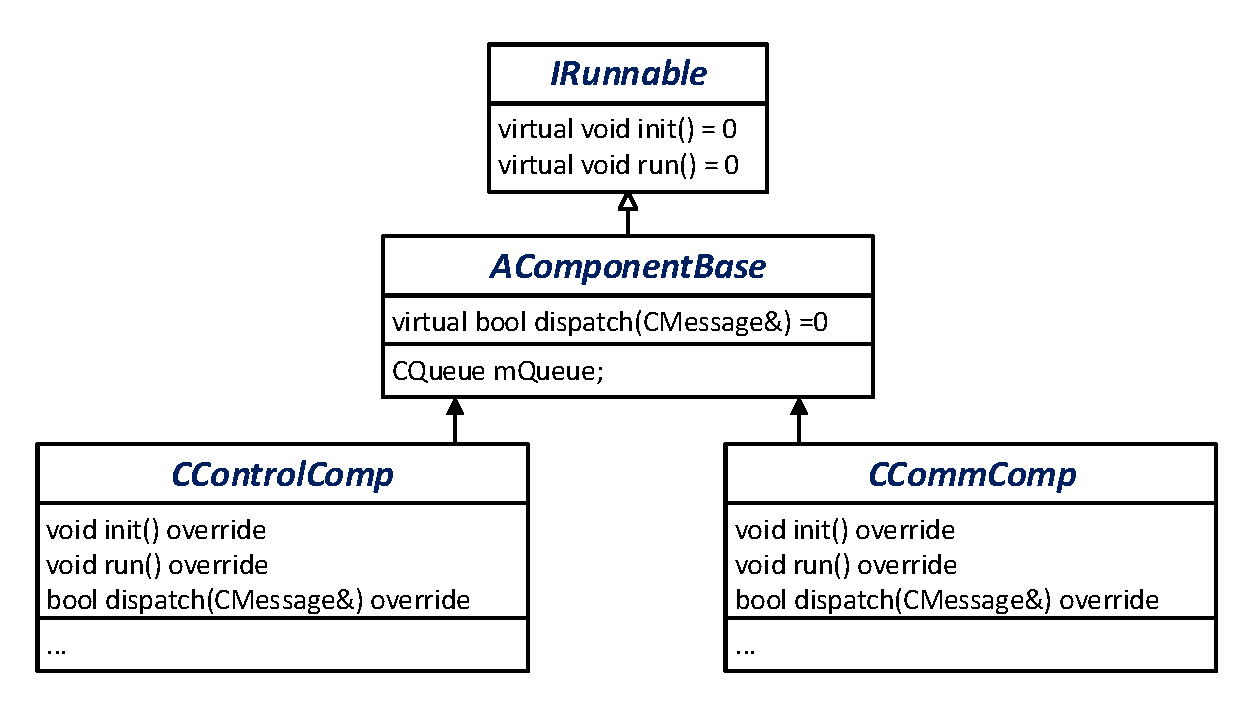
\includegraphics[width=0.6\linewidth]{img/SW_1_KA_KD.pdf}
\caption{Klassendiagramm der Komponenten}
\end{figure}

Im nächsten Schritt muss ein Weg zum Datenaustausch zwischen den Komponenten etabliert werden. Einerseits müssen Messdaten und Signale aus dem Regelkreis von der Regelungs- and die Kommunikationseinheit gesendet werden, welche diese anschließend an den Host-PC weiterleitet, andererseits werden die Steuerbefehle des Host-PCs von der Kommunikationskomponente empfangen und an die Regelungskomponente weitergegeben. Da in diesem Anwendungsfall lediglich kleine Datenmengen versendet werden, erfolgt die Übermittlung durch Nachrichten \cite[S. 196]{Wietzke1}. Die Nachrichten werden in Form der Klasse \textit{CMessage} implementiert, welche aus einem Datenfeld, einem Ereignis und einem Zeitstempel komponiert werden. Das Ereignis wird als Enumeration realisiert und gibt den Inhalt der Daten bzw. den jeweiligen Befehl wieder. Der Zeitstempel gibt den Abtastzeitpunkt der Signale aus dem Regelkreis wieder. 
\begin{lstlisting}[caption={Beispielhafte Implementierung der Events und Nachrichten},captionpos=b]
enum class EEvent
{
	DEFAULT_IGNORE = 0,
	TIMER_TICK     = 1,
	STATE_DATA     = 2,
	...
}
class CMessage
{
public:
	EEvent getEvent() const;
	UInt8* getDataPtr();
	...
public:

private:
	static constexpr UInt32 sDataSize = 32U;

	EEvent  mEvent;
	Float32 mTime;	
	UInt8   mData[sDataSize];
};
\end{lstlisting}
Außerdem besitzt die Klasse \textit{CMessage}Methoden und Konstruktoren, um die Datenfelder entsprechend zu füllen und auszulesen. Um die Nachrichten zu empfangen, besitzen die Komponenten Eingangspuffer, welche als Queues implementiert werden. Die Erzeugung der Nachrichten wird von einem Proxy übernommen \cite[S. 285 ff.]{Wietzke1}, der Methoden für die unterschiedlichen Ereignisse bereitstellt. Zudem kennt der Proxy die Queues der Komponenten und legt neue Nachrichten, in Abhängigkeit von dem jeweiligen Event, in die Eingangspuffers des zugehörigen Empfängers.
\begin{lstlisting}[caption={Aufbau der Proxy-Klasse},captionpos=b]
class CProxy
{
	public:
		bool transmitStateVector(const StateVector& x);
		bool onTimerTick();
		bool onClientConnect();
		...
};
\end{lstlisting}
Mit Hilfe der Nachrichtenkommunikation kann auch das Ablaufschema der Komponenten verallgemeinert werden. Beim Starten der Threads erfolgt die Initialisierung der Komponenten über den Aufrauf ihrer \textit{init()}-Methode. Anschließend wird die \textit{run()}-Methode ausgeführt, welche in diesem Fall eine Endlosschleife darstellt. In einem Durchlauf wird geprüft, ob neue Nachrichten vorhanden sind. Falls dies zutrifft, wird die Nachricht über die \textit{dispatch()}-Methode verarbeitet. Andernfalls legt sich der Thread schlafen, bis neue Nachrichten zur Verfügung stehen. Hieraus ergeben sich zwei Vorteile. Einerseits werden die Komponenten nach einem einheitlichen Konzept entworfen, lediglich die Implementierung der \textit{init()}- und \textit{dispatch()}-Methode unterscheiden sich, andererseits wird durch die Synchronisation der Komponenten deren Laufzeit reduziert.